\documentclass[aspectratio=169]{beamer}

% --- Theme and Style ---
\usetheme{Madrid}
\usecolortheme{whale}
\usefonttheme{professionalfonts}

% --- Packages ---
\usepackage[utf8]{inputenc}
\usepackage[T1]{fontenc}
\usepackage[indonesian]{babel}
\usepackage{amsmath, amsfonts, amssymb}
\usepackage{graphicx}
\usepackage{booktabs}
\usepackage{tikz}
\usepackage{caption}
\usepackage{subcaption}
\usepackage{algorithm}
\usepackage{algpseudocode}

% --- Metadata ---
\title[Integrasi EPG  dan   VQE]{Integrasi Exact Potential Game dan  Variational Quantum Eigensolver untuk Optimasi Portofolio Hibrida}
\subtitle{Tugas Akhir - Econophysics  dan   Quantum Finance}
\author[Nama Anda]{Nama Anda} % Silakan ganti dengan nama lengkap
\institute[Institusi]{Pembimbing: Nama Pembimbing \\ \medskip Departemen Fisika \\ Universitas ...}
\date{\today}

\graphicspath{{../Images/}}

% --- Custom Colors (Optional) ---
\definecolor{primaryblue}{RGB}{0, 31, 63}
\setbeamercolor{palette primary}{bg=primaryblue, fg=white}
\setbeamercolor{titlelike}{parent=palette primary}

% --- Logo ---
%\logo{\includegraphics[height=1cm]{Images/logo_universitas.png}}

\begin{document}

% Slide 1: Judul
\begin{frame}
    \titlepage
\end{frame}

% Daftar Isi
\begin{frame}{Outline}
    \tableofcontents
\end{frame}

% --- Konten Modular ---
%%\section{Pendahuluan}

% Slide 2: 1.1 Latar Belakang - Limitasi Model Markowitz
\begin{frame}{1.1 Latar Belakang - Limitasi Model Markowitz}
    \begin{itemize}
        \item \textbf{Modern Portfolio Theory:} Model \textit{Mean-Variance} (MV) sebagai fondasi utama alokasi aset dan \textbf{Diversifikasi}.
        \item \textbf{Masalah Utama:}
        \begin{itemize}
            \item Asumsi distribusi \textit{return} yang normal dan stasioner seringkali tidak realistis.
            \item Ketidakmampuan menangkap anomali pasar dan ketergantungan non-linear selama krisis.
        \end{itemize}
        \item \textbf{Solusi:} Transformasi fungsi objektif ke dalam kerangka \textit{Quadratic Unconstrained Binary Optimization} (QUBO).
    \end{itemize}
    \begin{center}
        \textit{Saran Gambar: Grafik Efficient Frontier Klasik vs Realitas Pasar (Fat-tailed distribution).}
    \end{center}
\end{frame}

% Slide 3: 1.1 Latar Belakang - Pendekatan Ekonofisika
\begin{frame}{1.1 Latar Belakang - Pendekatan Ekonofisika}
    \begin{itemize}
        \item \textbf{Model Ising:} Memetakan fungsi biaya portofolio ke dalam struktur Hamiltonian sistem fisik.
        \item \textbf{Representasi Spin:} Aset dianalogikan sebagai \textit{spins} yang berinteraksi dalam kisi kristal.
        \item \textbf{Fenomena Herding:} Sinkronisasi keputusan investor dicerminkan melalui keselarasan orientasi \textit{spin}.
        \item \textbf{Tujuan:} Mencari konfigurasi energi terendah (\textit{ground state}) yang setara dengan alokasi modal paling efisien.
    \end{itemize}
    \begin{center}
        %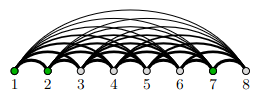
\includegraphics[width=0.4\textwidth]{Spin_Interaction_each.png} \\
        \textit{Saran Gambar: Visualisasi interaksi spin dalam kisi (Grid/Lattice).}
    \end{center}
\end{frame}

% Slide 4: 1.1 Latar Belakang - Integrasi Teori Permainan
\begin{frame}{1.1 Latar Belakang - Integrasi Teori Permainan}
    \begin{itemize}
        \item \textbf{Exact Potential Game (EPG):} Pemodelan interaksi strategis antar partisipan pasar secara dinamis.
        \item \textbf{Fungsi Potensial ($\Phi$):} Menjamin konsistensi antara utilitas marginal individu dan energi sistem total.
        \item \textbf{Kelebihan:} Deteksi bias aset secara presisi melalui pencarian titik \textit{Nash Equilibrium}.
        \item \textbf{Sinergi:} Integrasi EPG ke model Ising memodifikasi parameter medan lokal ($h_i$) berdasarkan logika permainan.
    \end{itemize}
\end{frame}

% Slide 5: 1.1 Latar Belakang - Strategi Warm-Start
\begin{frame}{1.1 Latar Belakang - Strategi Warm-Start}
    \begin{itemize}
        \item \textbf{Barren Plateaus:} Kendala lenyapnya gradien pada sirkuit kuantum variasional yang menghambat optimasi.
        \item \textbf{Warm-Start Strategis:} Memanfaatkan konfigurasi \textit{Nash Equilibrium} sebagai inisialisasi parameter awal VQE.
        \item \textbf{Mekanisme:} Menempatkan sirkuit pada wilayah probabilitas tinggi sejak iterasi pertama.
        \item \textbf{Hasil:} Mempercepat konvergensi energi menuju solusi optimal secara signifikan.
    \end{itemize}
\end{frame}

% Slide 6: 1.1 Latar Belakang - VQE dan Optimasi SPSA
\begin{frame}{1.1 Latar Belakang - VQE dan Optimasi SPSA}
    \begin{itemize}
        \item \textbf{Variational Quantum Eigensolver (VQE):} Algoritma hibrida yang fleksibel untuk perangkat keras era NISQ.
        \item \textbf{Optimasi SPSA:}
        \begin{itemize}
            \item Estimasi gradien efisien (hanya 2 pengukuran per iterasi).
            \item Tangguh terhadap \textit{noise} pengukuran dan fluktuasi statistik pasar.
        \end{itemize}
        \item \textbf{Ansatz EfficientSU(2):} Struktur sirkuit ringkas yang meminimalkan akumulasi \textit{gate noise} tanpa mengurangi ekspresivitas.
    \end{itemize}
\end{frame}

% Slide 7: 1.2 Rumusan Masalah
\begin{frame}{1.2 Rumusan Masalah}
    \begin{enumerate}
        \item Bagaimana perumusan bias aset ($h_i$) dan kopling ($J_{ij}$) menggunakan fungsi potensial EPG memengaruhi akurasi pemetaan Hamiltonian?
        \item Bagaimana efektivitas \textit{Nash Equilibrium} sebagai strategi \textit{warm-start} dalam mengatasi kendala inisialisasi algoritma VQE?
        \item Bagaimana performa algoritma VQE dengan optimasi SPSA dan \textit{Ansatz} EfficientSU(2) dalam menemukan solusi \textit{ground state}?
    \end{enumerate}
\end{frame}

% Slide 8: 1.3 Tujuan Penelitian
\begin{frame}{1.3 Tujuan Penelitian}
    \begin{enumerate}
        \item Menganalisis formulasi bias dan interaksi aset melalui pendekatan fungsi potensial EPG dalam sistem Hamiltonian.
        \item Mengevaluasi kontribusi strategi \textit{warm-start} berbasis \textit{Nash Equilibrium} dalam meningkatkan efisiensi pencarian solusi VQE.
        \item Menguji kapabilitas kombinasi VQE, SPSA, dan EfficientSU(2) untuk alokasi aset di pasar yang kompleks.
    \end{enumerate}
\end{frame}

% Slide 9: 1.4 Batasan Masalah
\begin{frame}{1.4 Batasan Masalah}
    \begin{itemize}
        \item \textbf{Portofolio:} Pemilihan aset dari pasangan sektor berbeda ($N=2$ dan $N=4$).
        \item \textbf{Model Game:} Skema \textit{non zero-sum game} dalam kerangka \textit{Exact Potential Game}.
        \item \textbf{Algoritma:} Pencarian ekuilibrium menggunakan \textit{Sequential Best Response} (SBR).
        \item \textbf{Implementasi:} Simulasi menggunakan framework \textit{PennyLane}.
    \end{itemize}
\end{frame}

% Slide 10: 1.5 Manfaat Penelitian
\begin{frame}{1.5 Manfaat Penelitian}
    \begin{itemize}
        \item Memberikan alternatif metode optimasi portofolio yang lebih tangguh terhadap dinamika korelasi pasar.
        \item Berkontribusi dalam literatur akademis mengenai penerapan komputasi kuantum pada bidang finansial (Econophysics).
        \item Menjembatani logika teori permainan dengan presisi optimasi mekanika kuantum.
    \end{itemize}
\end{frame}

%%\section{Landasan Konsep Finansial}

% Slide 4.1: Bab 2.1.1 - Evolusi Uang
\begin{frame}{Bab 2.1.1 - Evolusi Uang}
    \begin{itemize}
        \item Transformasi dari kebutuhan biologis (Barter) $\rightarrow$ Uang Komoditas (Logam) $\rightarrow$ Uang \textit{Fiat} $\rightarrow$ Entitas Data Digital.
    \end{itemize}
    \begin{figure}
        \centering
        \begin{subfigure}[b]{0.22\textwidth}
            \centering
            
\includegraphics[width=\textwidth]{211_Barter_marketeers.com.png}
            \caption{\textit{Barter}}
        \end{subfigure}
        \hfill
        \begin{subfigure}[b]{0.22\textwidth}
            \centering
            
\includegraphics[width=\textwidth]{211_Logam_depositphotos.com.png}
            \caption{\textit{Commodity}}
        \end{subfigure}
        \hfill
        \begin{subfigure}[b]{0.22\textwidth}
            \centering
            
\includegraphics[width=\textwidth]{211_Fiat_depositphotos.com.png}
            \caption{\textit{Fiat}}
        \end{subfigure}
        \hfill
        \begin{subfigure}[b]{0.22\textwidth}
            \centering
            
\includegraphics[width=\textwidth]{211_Digital_klasika.kompas.id.png}
            \caption{\textit{Digital}}
        \end{subfigure}
        \caption{Tahapan evolusi instrumen pertukaran nilai dalam peradaban manusia.}
    \end{figure}
\end{frame}

% Slide 4.2: Bab 2.1.2 - Inflasi
\begin{frame}{Bab 2.1.2 - Inflasi}
    \begin{columns}
        \begin{column}{0.5\textwidth}
            \begin{itemize}
                \item Fenomena sistemik peningkatan entropi ekonomi.
                \item Degradasi daya beli yang memaksa realokasi modal strategis untuk mempertahankan kekayaan riil.
            \end{itemize}
        \end{column}
        \begin{column}{0.5\textwidth}
            \begin{figure}
                \centering
                
\includegraphics[width=\textwidth]{212_Inflasi.png}
                \caption{Visualisasi dampak inflasi terhadap daya beli.}
            \end{figure}
        \end{column}
    \end{columns}
\end{frame}

% Slide 4.3: Bab 2.1.3 - Investasi
\begin{frame}{Bab 2.1.3 - Investasi}
    \begin{columns}
        \begin{column}{0.5\textwidth}
            \begin{itemize}
                \item Pengorbanan konsumsi jangka pendek untuk imbal hasil masa depan.
                \item Prinsip \textit{Risk-Return Trade-off}: Imbal hasil tinggi selalu diiringi risiko yang setara.
            \end{itemize}
        \end{column}
        \begin{column}{0.5\textwidth}
            \begin{figure}
                \centering
                
\includegraphics[width=0.8\textwidth]{213_Investasi.png}
                \caption{Spektrum risiko dan imbal hasil aset investasi.}
            \end{figure}
        \end{column}
    \end{columns}
\end{frame}

% Slide 4.4: Bab 2.1.4 - Penghindaran Risiko (Risk Aversion)
\begin{frame}{Bab 2.1.4 - Penghindaran Risiko (Risk Aversion)}
    \begin{columns}
        \begin{column}{0.5\textwidth}
            \begin{itemize}
                \item Parameter endogen yang dipengaruhi oleh Teori Prospek.
                \item Respon asimetris terhadap kerugian (\textit{loss aversion}) dibandingkan keuntungan.
            \end{itemize}
        \end{column}
        \begin{column}{0.5\textwidth}
            \begin{figure}
                \centering
                
\includegraphics[width=\textwidth]{214_RiskAversion_invespcro.com.png}
                \caption{Fungsi Utilitas dalam Teori Prospek.}
            \end{figure}
        \end{column}
    \end{columns}
\end{frame}

% Slide 5.1: Bab 2.2.1 - Analisis Kualitatif (Fundamental)
\begin{frame}{Bab 2.2.1 - Analisis Kualitatif (Fundamental)}
    \begin{columns}
        \begin{column}{0.5\textwidth}
            \begin{itemize}
                \item Evaluasi kesehatan industri dan emiten secara menyeluruh.
                \item Fokus pada laporan keuangan (\textit{Cashflow statement}), neraca, dan sentimen pasar.
                \item Menilai nilai intrinsik aset berdasarkan data makro dan mikro ekonomi.
            \end{itemize}
        \end{column}
        \begin{column}{0.5\textwidth}
            \begin{figure}
                \centering
                
\includegraphics[width=\textwidth]{221_Cashflow_statement.png}
                \caption{Komponen krusial dalam analisis fundamental.}
            \end{figure}
        \end{column}
    \end{columns}
\end{frame}

% Slide 5.2: Bab 2.2.2 - Analisis Teknikal (Visual)
\begin{frame}{Bab 2.2.2 - Analisis Teknikal (Visual)}
    \begin{itemize}
        \item Identifikasi pola memori kolektif pelaku pasar melalui representasi visual harga.
    \end{itemize}
    \begin{figure}
        \centering
        \begin{subfigure}[b]{0.3\textwidth}
            \centering
            
\includegraphics[width=\textwidth]{222_Candle.png}
            \caption{\textit{Candlestick}}
        \end{subfigure}
        \hfill
        \begin{subfigure}[b]{0.3\textwidth}
            \centering
            
\includegraphics[width=\textwidth]{222_Chart.png}
            \caption{\textit{Price Chart}}
        \end{subfigure}
        \hfill
        \begin{subfigure}[b]{0.3\textwidth}
            \centering
            
\includegraphics[width=\textwidth]{222_SnR.png}
            \caption{\textit{Support \& Resistance}}
        \end{subfigure}
        \caption{Instrumen utama dalam pemetaan psikologi pasar secara teknikal.}
    \end{figure}
\end{frame}

% Slide 5.3: Bab 2.2.3 - Analisis Kuantitatif
\begin{frame}{Bab 2.2.3 - Analisis Kuantitatif}
    \begin{columns}
        \begin{column}{0.5\textwidth}
            \begin{itemize}
                \item Transformasi harga mentah menjadi \textit{Log-Return} untuk mencapai stasioneritas data.
                \item Penting untuk pemodelan statistik dan input algoritma optimasi.
                \item Normalisasi rentang nilai guna kompatibilitas dengan sirkuit kuantum.
            \end{itemize}
        \end{column}
        \begin{column}{0.5\textwidth}
            \begin{figure}
                \centering
                
\includegraphics[width=\textwidth]{223_Price_log.png}
                \caption{Transformasi pergerakan harga menjadi deret imbal hasil (\textit{returns}).}
            \end{figure}
        \end{column}
    \end{columns}
\end{frame}

% Slide 5.4: Bab 2.2.4 - Optimasi Portofolio Markowitz
\begin{frame}{Bab 2.2.4 - Optimasi Portofolio Markowitz}
    \begin{columns}
        \begin{column}{0.5\textwidth}
            \begin{itemize}
                \item \textbf{Mean-Variance Optimization:} Mencari bobot aset ($\omega$) yang meminimalkan risiko untuk target imbal hasil tertentu.
                \item \textbf{Efficient Frontier:} Himpunan portofolio optimal yang menawarkan imbal hasil maksimal pada tingkat risiko tertentu.
            \end{itemize}
        \end{column}
        \begin{column}{0.5\textwidth}
            \begin{figure}
                \centering
                
\includegraphics[width=\textwidth]{224_Efficient_Frontier.png}
                \caption{Kurva batas efisiensi alokasi aset.}
            \end{figure}
        \end{column}
    \end{columns}
\end{frame}

%%\section{Teori Permainan dan Model Ising}

% Slide 6.1: Bab 2.3.1 - Pengantar Teori Permainan dan Ekuilibrium Nash
\begin{frame}{Bab 2.3.1 - Teori Permainan}
    \begin{itemize}
        \item Mengkaji bagaimana agen rasional membuat keputusan strategis di bawah ketergantungan agen yang lain.
        \item Terdiri dari beberapa unsur penting yaitu agen, himpunan strategi, dan fungsi utilitas.
        \item \textbf{\textit{Nash Equilibrium:}} Kondisi stabil di mana jika suatu agen mengubah strateginya maka agen tersebut akan mendapatkan utilitas yang lebih rendah.
        \item \textbf{Contoh Game:}
        \begin{enumerate}
            \item Stag Hunt
            \item Prisoner's Dilemma
            \item Battle of the Sexes
        \end{enumerate}
    \end{itemize}
    \begin{figure}
        \centering
        \begin{subfigure}[b]{0.3\textwidth}
            \centering
            
\includegraphics[width=\textwidth]{232_payoff_SH.png}
            \caption{\textit{Stag Hunt}}
        \end{subfigure}
        \hfill
        \begin{subfigure}[b]{0.15\textwidth}
            \centering
            
\includegraphics[width=\textwidth]{232_payoff_PD.png}
            \caption{\textit{Prisoner's Dilemma}}
        \end{subfigure}
        \hfill
        \begin{subfigure}[b]{0.3\textwidth}
            \centering
            
\includegraphics[width=\textwidth]{232_payoff_BoS.png}
            \caption{\textit{Battle of the Sexes}}
        \end{subfigure}
        \caption{Matriks \textit{payoff} klasik (Sumber: Referensi Teori Permainan).}
    \end{figure}
\end{frame}

% Slide 6.2: Bab 2.3.2 - Exact Potential Game (EPG)
\begin{frame}{Bab 2.3.2 - Exact Potential Game (EPG)}
    \begin{itemize}
        \item Merupakan permaianan yang menganggap utilitasnya sebagai fungsi potensial global $\Phi$.
        \item Berfungsi sebagai algoritma umum untuk mencari \textit{Nash Equilibrium} melalui maksimisasi fungsi potensial.
        \item Perubahan utilitas lokal ($\Delta u_i$) merepresentasikan perubahan potensial global ($\Delta \Phi$).
        \item Jika $\Delta \Phi > 0$, maka agen termotivasi untuk melakukan perubahan. Sebaliknya, jika $\Delta \Phi < 0$, maka agen akan menolak untuk melakukan perubahan sehingga didapatkan titik \textit{Nash Equilibrium}.
    \end{itemize}
    \begin{equation}
        \Delta \Phi = \Phi(s_i', s_{-i}) - \Phi(s_i, s_{-i}) = u_i(s_i', s_{-i}) - u_i(s_i, s_{-i})
    \end{equation}
    Dimana,
    \begin{itemize}
        \item $s_i$: Strategi agen $i$
        \item $s_{-i}$: Strategi agen selain agen $i$
        \item $u_i$: Utilitas agen $i$
        \item $u_i'$: Utilitas agen $i$ setelah melakukan perubahan
    \end{itemize}
\end{frame}

% Slide 6.3: Bab 2.3.3 - Penurunan Markowitz ke Kerangka EPG
\begin{frame}{Bab 2.3.3 - Dari Markowitz ke Kerangka EPG}
    \begin{itemize}
        \item \textbf{Transformasi Lagrangian Awal Menjadi Fungsi Potensial Global:}
        \begin{equation*}
            \begin{split}
                \Phi(\omega_i) &= -\frac{1}{\lambda} \mathcal{L}(\omega_i) \\
                &= -\sum_i \mu_i \omega_i + \frac{1}{\lambda} \sum_{i,j} \sigma_{ij} \omega_i \omega_j
            \end{split}
        \end{equation*}
        Dimana,
        \begin{itemize}
            \item $\lambda = \frac{\gamma}{2}$ dimana $\gamma$ merupakan parameter penentu tingkat penghindaran risiko (Risk Aversion) 
            \item $\sum_{i} \omega_i = 1$ yang mana jika ditransformasi ke variabel keputusan $x_i \in \{0, 1\}$, maka $\sum_{i} \omega_i = \frac{\sum_i x_i}{K} = 1$ dimana $K$ merupakan batas jumlah aset yang akan dipilih karena bobot diasumsikan sama rata.
        \end{itemize}
        \item Maka fungsi potensial EPG ($\Phi(x)$) menjadi:
        \begin{equation}
            \Phi(x) = \frac{1}{K} \sum_i \mu_i x_i - \frac{\gamma}{2K^2} \sum_{i,j} \sigma_{ij} x_i x_j
        \end{equation}
    \end{itemize}
\end{frame}

% Slide 7.1: Bab 2.4.1 - Sejarah dan Evolusi Model Ising
\begin{frame}{Bab 2.4.1 - Model Ising}
    \begin{itemize}
        \item \textbf{1920-an:} Wilhelm Lenz dan Ernst Ising merumuskan model interaksi spin diskrit.
        \item \textbf{1944:} Lars Onsager membuktikan transisi fase pada model Ising 2D.
        \item \textbf{Kontemporer:} Ising menjadi "bahasa standar" dalam optimasi kombinatorial karena kemajuan komputasi.
    \end{itemize}
    \begin{center}
        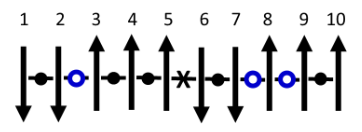
\includegraphics[width=0.5\textwidth]{1D_Model_atT.png} \\
        \footnotesize \textit{Model Ising 1D (Sumber: Figure 2.1 Bab 2).}
    \end{center}
\end{frame}

% Slide 7.2: Bab 2.4.2 - Transformasi QUBO
\begin{frame}{Bab 2.4.2 - Transformasi QUBO}
    \begin{itemize}
        \item Pemetaan fungsi EPG ke operator Hamiltonian: $\hat{H} = -\Phi(x)$
        \item Penurunan bentuk Hamiltonian objek menggunakan identitas $x_i^2 = x_i$
        {\tiny
        \begin{equation}
            \begin{split}
            \hat{H}_{obj}(x) &= \frac{\gamma}{2K^2}\sum_{i=1}^N\sum_{j=1}^N \sigma_{ij} x_i x_j - \sum_{i=1}^N \frac{\mu_i}{K} x_i \\
            &= \frac{\gamma}{2K^2}\left(\sum_{i=1}^N\sigma_i^2 x_i^2 + \sum_{i\ne j}\sigma_{ij} x_ix_j\right) -\sum_{i=1}^N \frac{\mu_i}{K} x_i \\
            &= \frac{\gamma}{2K^2}\sum_{i=1}^N\sigma_i^2 x_i^2 + \frac{\gamma}{2K^2}\sum_{i\ne j}\sigma_{ij} x_ix_j - \sum_{i=1}^N \frac{\mu_i}{K} x_i \\
            &= \frac{\gamma}{2K^2}\sum_{i=1}^N\sigma_i^2 x_i + \frac{\gamma}{2K^2}\sum_{i\ne j}\sigma_{ij} x_ix_j - \sum_{i=1}^N \frac{\mu_i}{K} x_i \\
            &= \sum_{i=1}^N\left(\frac{\gamma \sigma_i^2}{2K^2} - \frac{\mu_i}{K}\right)x_i + \sum_{i\ne j}\frac{\gamma \sigma_{ij}}{2K^2} x_ix_j
            \end{split}
        \end{equation}
        }
    \end{itemize}
\end{frame}

\begin{frame}{Bab 2.4.2 - Transformasi QUBO (Lanjutan)}
    \begin{itemize}
        \item Penambahan suku penalti untuk kendala $\sum x_i = K$:
        {\tiny
        \begin{equation}
            \begin{split}
            \hat{H}_{pen}(x) &= A\left(\sum_{i=1}^N x_i - K\right)^2 \\
            &= A\left(\sum_{i=1}^N x_i^2 + \sum_{i\ne j} x_ix_j - 2K\sum_{i=1}^N x_i + K^2\right) \\
            &= A\sum_{i=1}^N x_i^2 + A\sum_{i\ne j} x_ix_j - 2AK\sum_{i=1}^N x_i + AK^2
            \end{split}
        \end{equation}
        }
        \item Hamiltonian total diperoleh dengan menggabungkan fungsi Hamiltonian objek dengan fungsi penalti:
        {\tiny
        \begin{equation}
            \begin{split}
                \hat{H} =& \hat{H}_{obj} (x) + \hat{H}_{pen} (x) \\
                =& \sum_i \left(\frac{\gamma \sigma_i^2}{2K^2} - \frac{\mu_i}{K}\right)x_i + \sum_{i\ne j}\frac{\gamma \sigma_{ij}}{2K^2} x_ix_j  + A\sum_{i=1}^N x_i^2 + A\sum_{i\ne j} x_ix_j - 2AK\sum_{i=1}^N x_i + AK^2 \\
                =& \sum_i \left(\frac{\gamma \sigma_i^2}{2K^2} + A - \frac{\mu_i}{K} - 2AK\right)x_i + \sum_{i\ne j}\left(\frac{\gamma \sigma_{ij}}{2K^2} + A\right) x_ix_j + AK^2
            \end{split}
        \end{equation}
        }
    \end{itemize}
\end{frame}

\begin{frame}{Bab 2.4.2 - Transformasi QUBO (Lanjutan)}
    \begin{itemize}
        \item Jika dimisalkan
        {\tiny
        \begin{equation*}
            Q_{ii} = \frac{\gamma \sigma_i^2}{2K^2} + A - \frac{\mu_i}{K} - 2AK \quad \text{dan} \quad Q_{ij} = \frac{\gamma \sigma_{ij}}{2K^2} + A
        \end{equation*}
        }
        \item Persamaan QUBO dapat disederhanakan menjadi
        {\tiny
        \begin{equation}
            \hat{H} = \sum_i Q_{ii} x_i + \sum_{i\ne j} Q_{ij} x_ix_j + AK^2
        \end{equation}
        }
        \item Substitusi variabel keputusan $x_i \in \{0, 1\}$ ke spin $\hat{Z}_i \in \{-1, 1\}$
        {\tiny
        \begin{equation}
            \begin{split}
                x_i     &= \frac{1 - \hat{Z}_i}{2} \\
                x_ix_j  &= \frac{1 - \hat{Z}_i - \hat{Z}_j + \hat{Z}_i \hat{Z}_j}{4}
            \end{split}
        \end{equation}
        }
        sehingga menjadi
        {\tiny
        \begin{equation}
            \begin{split}
                \hat{H} &= \sum_i Q_{ii} \left(\frac{1 - \hat{Z}_i}{2}\right) + \sum_{i\ne j} Q_{ij} \left(\frac{1 - \hat{Z}_i - \hat{Z}_j + \hat{Z}_i \hat{Z}_j}{4}\right) + AK^2 \\
                \hat{H} &= \sum_i Q_{ii} \frac{1}{2} - \sum_i Q_{ii} \frac{\hat{Z}_i}{2} + \sum_{i\ne j} Q_{ij} \frac{1}{4} - \sum_{i\ne j} Q_{ij} \frac{\hat{Z}_i}{4} - \sum_{i\ne j} Q_{ij} \frac{\hat{Z}_j}{4} + \sum_{i\ne j} Q_{ij} \frac{\hat{Z}_i \hat{Z}_j}{4} + AK^2 \\
                \hat{H} &= \sum_i \left(- \frac{Q_{ii}}{2} - \sum_{i\ne j} \frac{Q_{ij}}{2}\right) \hat{Z}_i + \sum_{i\ne j} \frac{Q_{ij}}{4} \hat{Z}_i \hat{Z}_j + \left(\sum_i \frac{Q_{ii}}{2} + \sum_{i\ne j} \frac{Q_{ij}}{4} + AK^2\right) \quad \text{karena } Q_{ij} = Q_{ji}
            \end{split}
        \end{equation}
        }
    \end{itemize}
\end{frame}

\begin{frame}{Bab 2.4.2 - Transformasi QUBO (Lanjutan)}
    \begin{itemize}
        \item Bisa kita dapatkan
        \begin{equation*}
            h_i = - \frac{Q_{ii}}{2} - \sum_{i\ne j} \frac{Q_{ij}}{2}
        \end{equation*}
        \begin{equation*}
            J_{ij} = \frac{Q_{ij}}{4}
        \end{equation*}
        \begin{equation*}
            C = \sum_i \frac{Q_{ii}}{2} + \sum_{i\ne j} \frac{Q_{ij}}{4} + AK^2
        \end{equation*}
        \begin{equation*}
            \hat{H} = - \sum_i h_i \hat{Z}_i - \sum_{i<j} J_{ij} \hat{Z}_i \hat{Z}_j + C
        \end{equation*}
        \item \textbf{Dimana;}
        \begin{itemize}
            \item $h_i$ merupakan koefisien interaksi spin dengan fluktuasi pasar.
            \item $J_{ij}$ merupakan koefisien interaksi antar-spin yang bergantung pada kovariansi.
            \item $C$ merupakan konstanta.
        \end{itemize}
    \end{itemize}
\end{frame}

%%\section{Komputer Kuantum}

% Slide 8.1: Bab 2.5.1 - Dari Bit Klasik ke Qubit Kuantum
\begin{frame}{Bab 2.5.1 - Dari Bit Klasik ke Qubit Kuantum}
    \begin{columns}
        \begin{column}{0.5\textwidth}
            \textbf{Bit Klasik:}
            \begin{itemize}
                \item Unit informasi fundamental komputer konvensional.
                \item Bersifat deterministik: hanya bernilai 0 atau 1.
                \item 0 berarti tidak ada arus listrik, 1 berarti ada arus listrik
            \end{itemize}
        \end{column}
        \begin{column}{0.5\textwidth}
            \textbf{Qubit Kuantum:}
            \begin{itemize}
                \item Unit informasi fundamental komputer kuantum.
                \item Memanfaatkan prinsip Superposisi: 0, 1, atau keduanya.
                \item $|\psi\rangle = \alpha|0\rangle + \beta|1\rangle$
            \end{itemize}
        \end{column}
    \end{columns}
\end{frame}

% Slide 8.2: Bab 2.5.2 - Representasi Matriks Qubit
\begin{frame}{Bab 2.5.2 - Representasi Matriks Qubit}
    \begin{itemize}
        \item Status qubit didefinisikan sebagai vektor kolom di ruang Hilbert kompleks.
        \item \textbf{Basis Komputasi:}
        \begin{equation*}
            |0\rangle = \begin{pmatrix} 1 \\ 0 \end{pmatrix}, \quad |1\rangle = \begin{pmatrix} 0 \\ 1 \end{pmatrix}
        \end{equation*}
        \item \textbf{Aturan Born (Born Rule):} Probabilitas menemukan sistem pada status $i$ adalah $P(i) = |\langle i | \psi \rangle|^2$.
        dimana
        \begin{itemize}
            \item $|\psi\rangle$ adalah keadaan sistem kuantum sebelum diukur
            \item $|i\rangle$ adalah keadaan sistem kuantum setelah diukur
            \item $\langle i | \psi \rangle$ adalah amplitudo probabilitas.
            \item $|\langle i | \psi \rangle|^2$ adalah probabilitas menemukan sistem pada status $i$.
        \end{itemize}
        \item Dengan syarat normalisasi total probabilitas harus bernilai 1 ($|\alpha|^2 + |\beta|^2 = 1$).
    \end{itemize}
\end{frame}

% Slide 8.3: Bab 2.5.3 - Geometri Qubit: Bola Bloch
\begin{frame}{Bab 2.5.3 - Geometri Qubit: Bola Bloch}
    \begin{columns}
        \begin{column}{0.6\textwidth}
            \begin{itemize}
                \item Keadaan kuantum dapat direpresentasikan ke dalam visualisasi Bola Bloch.
                \item Terdapat 2 parameter sudut pada bola bloch
                \begin{itemize}
                    \item $\theta$ (Polar): Menentukan probabilitas $|0\rangle$ vs $|1\rangle$.
                    \item $\phi$ (Azimuthal): Menentukan fase kuantum.
                \end{itemize}
                \item Sehingga fungsi gelombang qubit dapat dinyatakan sebagai
                \begin{equation*}
                    |\psi\rangle = \cos\frac{\theta}{2}|0\rangle + e^{i\phi}\sin\frac{\theta}{2}|1\rangle.
                \end{equation*}
            \end{itemize}
        \end{column}
        \begin{column}{0.4\textwidth}
            \begin{center}
                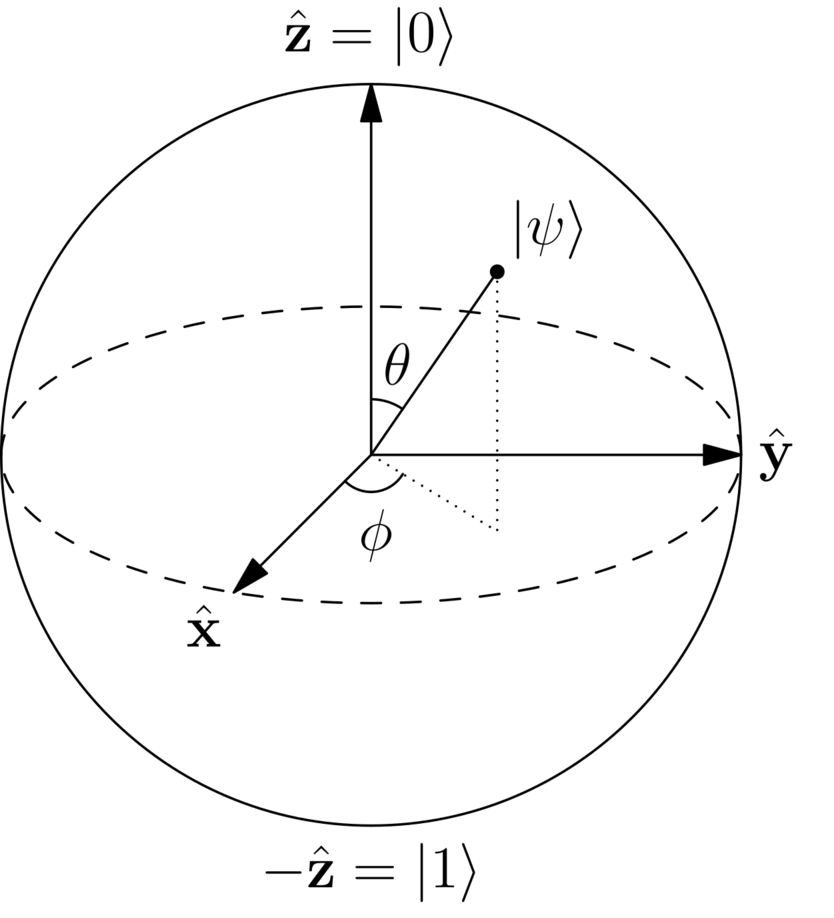
\includegraphics[width=0.8\textwidth]{bloch_sphere.png} \\
                \footnotesize \textit{Sumber: Qiskit Documentation}
            \end{center}
        \end{column}
    \end{columns}
\end{frame}

% Slide 8.4: Bab 2.5.4 - Gerbang Rotasi Kuantum
\begin{frame}{Bab 2.5.4 - Gerbang Rotasi Kuantum}
    \begin{itemize}
    \item Gerbang kuantum merupakan operator unitari yang digunakan untuk memanipulasi status qubit dengan dasar matriks pauli
    \begin{equation}
        \sigma_x = \begin{pmatrix} 0 & 1 \\ 1 & 0 \end{pmatrix}, \quad \sigma_y = \begin{pmatrix} 0 & -i \\ i & 0 \end{pmatrix}, \quad \sigma_z = \begin{pmatrix} 1 & 0 \\ 0 & -1 \end{pmatrix}
    \end{equation}
    \item Dengan rumus dasar $R_{\sigma}(\theta) = e^{-i \frac{\theta}{2} \sigma} = \cos\frac{\theta}{2} I - i \sin\frac{\theta}{2} \sigma$, maka bentuk matriks dari gerbang rotasi qubit adalah
    {\tiny
    \begin{equation}
        R_x(\theta) = \begin{pmatrix} \cos\frac{\theta}{2} & -\sin\frac{\theta}{2} \\ \sin\frac{\theta}{2} & \cos\frac{\theta}{2} \end{pmatrix}, \quad R_y(\theta) = \begin{pmatrix} \cos\frac{\theta}{2} & -\sin\frac{\theta}{2} \\ \sin\frac{\theta}{2} & \cos\frac{\theta}{2} \end{pmatrix}, \quad R_z(\phi) = \begin{pmatrix} e^{-i\phi/2} & 0 \\ 0 & e^{i\phi/2} \end{pmatrix}.
    \end{equation}
    }
    \end{itemize}
\end{frame}

% Slide 8.5: Bab 2.5.5 - Gerbang Keterbelitan (Entanglement)
\begin{frame}{Bab 2.5.5 - Gerbang Keterbelitan (Entanglement)}
    \begin{columns}
        \begin{column}{0.5\textwidth}
            \begin{itemize}
        \item \textbf{Interaksi Non-Lokal:} Status satu qubit menjadi bergantung pada qubit lainnya.
        \item \textbf{Gerbang CNOT:} Membalik fasa qubit target jika qubit kontrol bernilai 1.
        \item sebagai contoh qubit 0 sebagai kontrol dan qubit 1 sebagai target, maka
        \begin{equation*}
            \begin{split}
                \text{CNOT}_{01} \quad &|00\rangle \to |00\rangle \\
                &|01\rangle \to |01\rangle \\
                &|10\rangle \to |11\rangle \\
                &|11\rangle \to |10\rangle
            \end{split}
        \end{equation*}
    \end{itemize}
        \end{column}
        \begin{column}{0.5\textwidth}
            \begin{itemize}
                \item Dimana bentuk matriks setiap keadaan
                \begin{equation*}
                    \begin{aligned}
                        |00\rangle &= \begin{pmatrix} 1 & 0 & 0 & 0 \end{pmatrix}^T \\ 
                        |01\rangle &= \begin{pmatrix} 0 & 1 & 0 & 0 \end{pmatrix}^T \\
                        |10\rangle &= \begin{pmatrix} 0 & 0 & 1 & 0 \end{pmatrix}^T \\
                        |11\rangle &= \begin{pmatrix} 0 & 0 & 0 & 1 \end{pmatrix}^T
                    \end{aligned}
                \end{equation*}
                \item Perubahan tersebut dapat disatukan dalam bentuk matriks 
            \end{itemize}
            \begin{equation*}
            \text{CNOT}_{01} = \begin{pmatrix} 1 & 0 & 0 & 0 \\ 0 & 1 & 0 & 0 \\ 0 & 0 & 0 & 1 \\ 0 & 0 & 1 & 0 \end{pmatrix}
        \end{equation*}
        \end{column}
    \end{columns}
\end{frame}

% Slide 8.6: Bab 2.5.6 - Parameterized Quantum Circuit (PQC)
\begin{frame}{Bab 2.5.6 - Parameterized Quantum Circuit (PQC)}
    \begin{itemize}
        \item Sirkuit kuantum berparameter (PQC) merupakan rangkaian gerbang kuantum yang nilai parameternya ($\boldsymbol{\theta}$) dapat diatur.
        \item Sirkuit kuantum berparameter (PQC) terdiri dari \textit{Data Encoding}, \textit{Variational Layers}, dan \textit{Measurement}
        \item Lalu pengukuran energi dievaluasi oleh optimasi klasik untuk dicari parameter barunya sampai
    \end{itemize}
    \begin{center}
        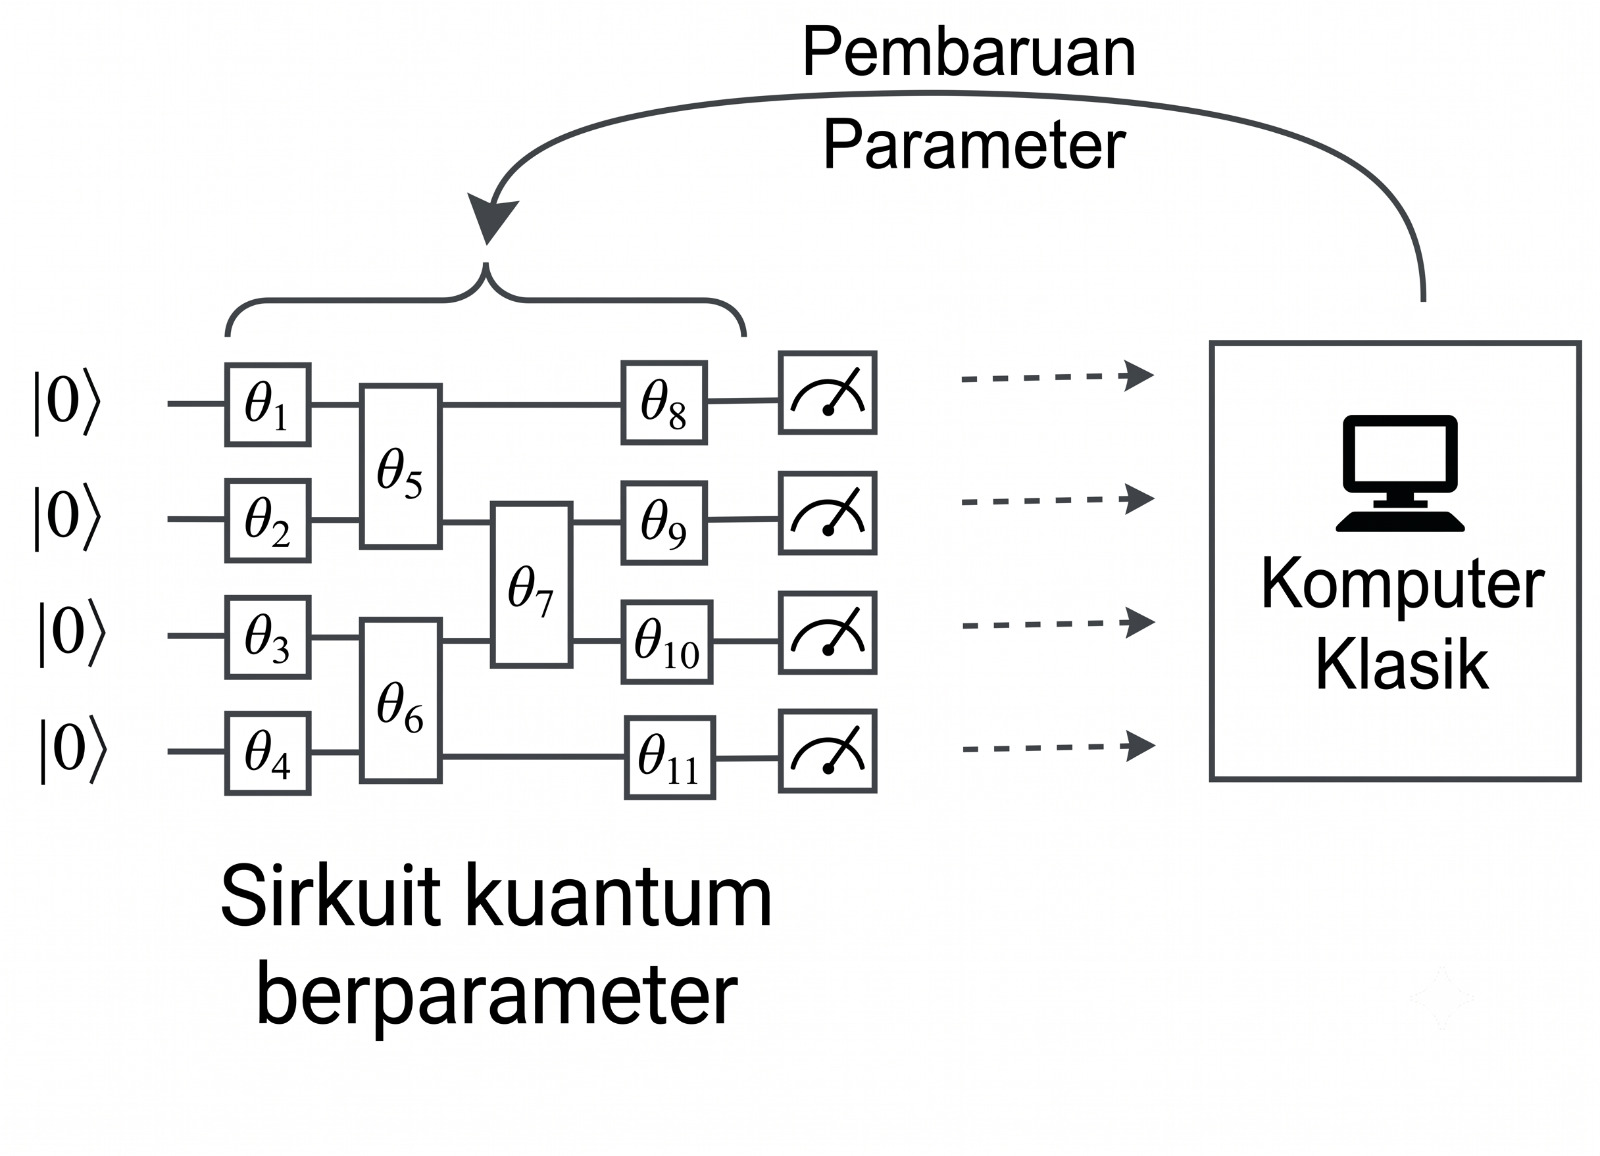
\includegraphics[width=0.4\textwidth]{Gambar/256_PQC1.jpeg} \\
    \end{center}
\end{frame}

%%\section{Optimasi dan VQE}

% Slide 9.1: Bab 2.6.1 - Gradien Energi
\begin{frame}{Bab 2.6.1 - Gradien Energi}
    \begin{itemize}
        \item Pembaruan parameter menggunakan nilai dari gradien energi
        \begin{equation}
            \frac{\partial E}{\partial \theta} = \frac{\langle\psi(\theta)|\hat{H}|\psi(\theta)\rangle}{\partial \theta}
        \end{equation}
        \item Misal sistem memliki 2 qubit, maka 
        \begin{equation}
            \begin{split}
            \frac{\partial E}{\partial \theta} &= \frac{\bra{00} \hat{U}_{A}^\dagger \hat{U}(\theta)^\dagger \hat{U}_{B}^\dagger \hat{\mathcal{H}} \hat{U}_{B} \hat{U}(\theta) \hat{U}_{A} \ket{00}}{\partial \theta} \\
            &= \frac{\bra{\phi} \hat{U}(\theta)^\dagger \hat{U}_{B}^\dagger \hat{\mathcal{H}} \hat{U}_{B} \hat{U}(\theta) \ket{\phi}}{\partial \theta} \\
            &= \frac{\bra{\phi} \hat{U}(\theta)^\dagger \hat{M} \hat{U}(\theta) \ket{\phi}}{\partial \theta}
            \end{split}
        \end{equation}
    \end{itemize}
\end{frame}

\begin{frame}{Bab 2.6.1 - Gradien Energi Lanjutan}
    \begin{itemize}
        \item dengan turunan uniter
        \begin{equation*}
            \frac{\partial U(\theta)}{\partial\theta} = -\frac{i}{2}\sigma(\theta) U(\theta) \quad \text{dan} \quad \frac{\partial U^\dagger(\theta)}{\partial\theta} = \frac{i}{2}\sigma(\theta) U^\dagger(\theta)
        \end{equation*}
    \item maka turunan menjadi 
    {\tiny
    \begin{equation*}
        \begin{split}
        \frac{\partial \langle E(\theta)\rangle}{\partial \theta} &= \bra{\phi} \frac{\partial U^{\dagger}(\theta)}{\partial \theta} M U(\theta) \ket{\phi} + \bra{\phi} U^{\dagger}(\theta) M \frac{\partial U(\theta)}{\partial \theta} \ket{\phi} \\
        &= \bra{\phi} \left(\frac{i}{2}\sigma U^{\dagger}(\theta)\right) M U(\theta) \ket{\phi} + \bra{\phi} U^{\dagger}(\theta) M \left(-\frac{i}{2}\sigma U(\theta)\right) \ket{\phi} \\
        &= \frac{i}{2} \bra{\psi(\theta)} \sigma M \ket{\psi(\theta)} - \frac{i}{2} \bra{\psi(\theta)} M \sigma \ket{\psi(\theta)} \\
            &= \frac{i}{2} \bra{\psi(\theta)} \sigma M - M \sigma \ket{\psi(\theta)}
        \end{split}
    \end{equation*}
    }
    \item sehingga didapatkan
        \begin{equation}
        \frac{\partial \langle E(\theta)\rangle}{\partial \theta} = \frac{i}{2} \bra{\psi(\theta)} [\sigma, M] \ket{\psi(\theta)}
        \end{equation}
\end{itemize}
\end{frame}

% Slide 9.2: Bab 2.6.2 - Parameter Shift Rule (PSR)
\begin{frame}{Bab 2.6.2 - Parameter Shift Rule (PSR)}
    \begin{itemize}
        \item PSR menggunakan konsep pergeseran parameter $\theta$ sebesar $s = \frac{\pi}{2}$ ke arah positif dan negatif
        \begin{equation}
            \begin{split}
            \hat{U}(\theta \pm s) &= \exp\left(-i\frac{\theta \pm s}{2}\sigma\right) \\
            &= \exp\left(-i\frac{\theta}{2}\sigma\right) \exp\left(\mp i\frac{s}{2}\sigma\right) \\
            &= \hat{U}(\theta) \hat{U}(\pm s).
            \end{split}
        \end{equation}
        \item sehingga ekspektasi energi menjadi
        \begin{equation*}
            \begin{split}
            \langle E(\theta\pm s)\rangle &= \bra{\phi}\hat{U}(\theta\pm s)^{\dagger}\hat{M}\hat{U}(\theta\pm s)|\phi\rangle \\
            &= \bra{\phi}\hat{U}(\theta)^{\dagger}\hat{U}(\pm s)^{\dagger}\hat{M}\hat{U}(\theta)\hat{U}(\pm s)|\phi\rangle \\
            &= \bra{\psi} \hat{U}(\pm s)^{\dagger}\hat{M}\hat{U}(\pm s)|\psi\rangle.
            \end{split}
        \end{equation*}
    \end{itemize}
\end{frame}

\begin{frame}{Bab 2.6.2 - Parameter Shift Rule (PSR)}
    \begin{itemize}
        \item sehingga untuk pergeseran positif
        {\tiny
        \begin{equation}
            \begin{split}
                \langle E(\theta+s)\rangle = \bra{\psi(\theta)} & \left[ \cos\left(\frac{s}{2}\right) \hat{I} + i \sin\left(\frac{s}{2}\right) \sigma \right] \hat{M} \left[ \cos\left(\frac{s}{2}\right) \hat{I} - i \sin\left(\frac{s}{2}\right) \sigma \right] \ket{\psi(\theta)} \\
                = \bra{\psi(\theta)} & \left[ \cos^2\left(\frac{s}{2}\right) \hat{M} - i \cos\left(\frac{s}{2}\right) \sin\left(\frac{s}{2}\right) \hat{M} \sigma + \right. \\
                & \left. i \sin\left(\frac{s}{2}\right) \cos\left(\frac{s}{2}\right) \sigma \hat{M} + \sin^2\left(\frac{s}{2}\right) \sigma \hat{M} \sigma \right] \ket{\psi(\theta)}.
            \end{split}
        \end{equation}
        \begin{equation}
            \begin{split}
            \langle E(\theta+s)\rangle = &\cos^2\left(\frac{s}{2}\right) \langle \hat{M} \rangle + \sin^2\left(\frac{s}{2}\right) \langle\sigma \hat{M} \sigma\rangle + i \sin\left(\frac{s}{2}\right) \cos\left(\frac{s}{2}\right) \langle [\sigma, \hat{M}] \rangle.
            \end{split}
        \end{equation}
        \begin{equation}
            \begin{split}
            \langle E(\theta-s)\rangle = &\cos^2\left(\frac{s}{2}\right) \langle \hat{M} \rangle + \sin^2\left(\frac{s}{2}\right) \langle\sigma \hat{M} \sigma\rangle - i \sin\left(\frac{s}{2}\right) \cos\left(\frac{s}{2}\right) \langle [\sigma, \hat{M}] \rangle.
            \end{split}
        \end{equation}
        }
        \item dengan menghitung selisih kedua pergeserang tersebut, maka didapatkan;
        \begin{equation}
            \begin{split}
                \langle E(\theta+s)\rangle - \langle E(\theta-s)\rangle &= 2 i \sin\left(\frac{s}{2}\right) \cos\left(\frac{s}{2}\right) \langle [\sigma, \hat{M}] \rangle \\
                &= i \sin(s) \langle [\sigma, \hat{M}] \rangle.
            \end{split}
        \end{equation}
    \end{itemize}
\end{frame}

\begin{frame}{Bab 2.6.2 - Parameter Shift Rule (PSR)}
    \begin{itemize}
        \item Jika $s = \frac{\pi}{2}$, maka $\sin(s) = 1$ dan $\cos(s) = 0$, sehingga didapatkan persamaan umum parameter shift rule
        \begin{equation*}
            \begin{split}
                2 \frac{\partial \langle E(\theta)\rangle}{\partial \theta} &= i \langle [\sigma, M]\rangle \\
                2 \frac{\partial \langle E(\theta)\rangle}{\partial \theta} &= \langle E(\theta+s)\rangle - \langle E(\theta-s)\rangle \\
            \end{split}
        \end{equation*}
        \begin{equation}
            \frac{\partial \langle E(\theta)\rangle}{\partial \theta} = \frac{1}{2} \left[ \langle E(\theta+s)\rangle - \langle E(\theta-s)\rangle \right]
        \end{equation}
    \end{itemize}
\end{frame}

% Slide 9.3: Bab 2.6.3 - Gradient Descent (GD)
\begin{frame}{Bab 2.6.3 - Gradient Descent (GD)}
    \begin{itemize}
        \item \textbf{Mekanisme:} Parameter $\theta$ diperbarui searah negatif gradien untuk mencapai minimum energi.
        \begin{equation*}
            \theta_{t+1} = \theta_t - \eta \nabla E(\theta_t)
        \end{equation*}
        \item dimana 
        \begin{itemize}
            \item $\theta_{t+1}$ adalah parameter pada iterasi ke $t+1$
            \item $\eta$ adalah laju pembelajaran 
            \item $\nabla E(\theta_t)$ adalah gradien energi pada parameter $\theta_t$.
        \end{itemize}
        \item \textbf{Kekurangan:} Harus mengevaluasi gradien dua kali untuk setiap parameter, sehingga kompleksitas evaluasi gradien PSR tumbuh linear terhadap jumlah parameter.
    \end{itemize}
\end{frame}

% Slide 9.4: Bab 2.6.4 - Optimizer SPSA
\begin{frame}{Bab 2.6.4 - Optimizer SPSA}
    \begin{itemize}
        \item \textbf{Inovasi:} Estimasi gradien seluruh parameter secara simultan menggunakan vektor perturbasi acak ($\pm 1$).
        {\tiny
        \begin{equation}
            \begin{split}
                E_{\pm} &= E(\theta_k \pm c_k \Delta_k) \\ 
                &\approx E(\theta_k) \pm c_k \sum_{j=1}^p \Delta_j \frac{\partial E}{\partial \theta_j} + \frac{1}{2} c_k^2 \sum_{j=1}^p \Delta_j^2 \frac{\partial^2 E}{\partial \theta_j^2} + \dots
            \end{split}
        \end{equation}
        }
        \item Sehingga jika diambil selisih kedua evaluasi tersebut,
        {\tiny
        \begin{equation}
            \begin{split}
                E_+ - E_- &= 2 c_k \sum_{j=1}^p \Delta_j \frac{\partial E}{\partial \theta_j} + O(c_k^3)
            \end{split}
        \end{equation}
        }
        \item maka didapatkan bentuk estimator gradien
        {\tiny
        \begin{equation}
            \begin{split}
                \hat{g}_i &= \frac{E_+ - E_-}{2 c_k \Delta_i} \\
                &= \frac{1}{\Delta_i} \sum_{j=1}^p \Delta_j \frac{\partial E}{\partial \theta_j} \\
                &= \frac{\Delta_i}{\Delta_i} \frac{\partial E}{\partial \theta_i} + \sum_{j \neq i} \frac{\Delta_j}{\Delta_i} \frac{\partial E}{\partial \theta_j} \\
                \mathbb{E} \left[ \hat{g}_i \right] &= \frac{\partial E}{\partial \theta_i} + \sum_{j \neq i} \mathbb{E} \left[ \frac{\Delta_j}{\Delta_i} \right] \frac{\partial E}{\partial \theta_j}
            \end{split}
        \end{equation}
        }
    \end{itemize}
\end{frame}

\begin{frame}{Bab 2.6.4 - Optimizer SPSA}
    \begin{itemize}
        \item Sehingga dekspektasi estimasi gradien
        \begin{equation}
            \mathbb{E} \left[ \hat{g}_i \right] = \frac{\partial E}{\partial \theta_i}
        \end{equation} 
        \item  dengan proses optimasi 
        \begin{equation}
            \theta_{k+1} = \theta_k - \eta \hat{g}_k
        \end{equation}
        \item dengan 
        \begin{itemize}
            \item $c_k$ merupakan koefisien perturbasi yang menurun seiring dengan iterasi 
            \item $\eta$ merupakan laju pembelajaran 
            \item $\hat{g}_k$ merupakan estimasi gradien pada iterasi ke $k$
        \end{itemize}
        \item SPSA lebih efisien dibandingkan GD karena hanya membutuhkan 50\% evaluasi fungsi biaya pada setiap iterasi dari GD
    \end{itemize}
\end{frame}

% Slide 10.2: Bab 2.7 - Arsitektur EfficientSU2 (HEA)
\begin{frame}{Bab 2.7 - VQE dengan Arsitektur EfficientSU2 (HEA)}
    \begin{itemize}
        \item Menggunakan prinsip variasi Reyleigh-Ritz yang menyatakan bahwa energi dari status percobaan selalu lebih besar atau sama dengan energi \textit{ground state} sejati ($E_0$).
        \begin{equation*}
            E(\theta) = \frac{\langle\psi(\theta)|\hat{H}|\psi(\theta)\rangle}{\langle\psi(\theta)|\psi(\theta)\rangle} \ge E_0
        \end{equation*}
        \item Menggunakan struktur lapisan rotasi ($R_y, R_z$) dan lapisan keterbelitan (\textit{entanglement}) menggunakan gerbang CNOT.
    \end{itemize}
    \begin{center}
        
\includegraphics[width=0.6\textwidth]{../GTQuantumInvest/Hasil_N2_GT/Analisis_Window_N2/2021-05-05_circuit.png}
    \end{center}
\end{frame}

% Slide 11.1: Bab 2.8.1 - Fenomena Barren Plateau
\begin{frame}{Bab 2.8.1 - Fenomena Barren Plateau dan Keacakan}
    \begin{itemize}
        \item Semakin tinggi \textbf{kedalaman sirkuit} = semakin besar \textbf{ekspresibilitas} = semakin besar risiko terjebak pada \textbf{Barren Plateau}
        \item \textbf{Barren Plateau} ditandai oleh lenyapnya varians gradien karena  
        \begin{equation}
            \text{Var}[\partial_{\theta} E] \propto \frac{1}{2^{NL}}
        \end{equation}
        dimana N adalah jumlah qubit dan L adalah kedalaman sirkuit
        \item Untuk mengkuran keacakan keadaaan kuantum selama optimasi, digunakan entropi von Neumann
        \begin{equation}
            S(\rho) = -\text{Tr}(\rho \log \rho)
        \end{equation}
        dimana $\rho$ merupakan matriks densitas dari keadaan kuantum
    \end{itemize}
\end{frame}

% Slide 11.2: Bab 2.8.2 - Diagnostik: Entropi Von Neumann
\begin{frame}{Bab 2.8.2 - Entropi Von Neumann dan Entropi Shannon}
    \begin{itemize}
        \item Mengukur derajat kemurnian state kuantum selama optimasi
        \item Berawal dari entopi Shannon, 
    \end{itemize}
    {\scriptsize
    \begin{equation*}
        \begin{split}
            H &= - \sum_i p_i \log_2 (p_i) \\
            \rho &= \sum_i p_i |\psi_i\rangle \langle \psi_i| \\
            \rho &= \sum_j \lambda_j |e_j\rangle \langle e_j| \\
            \log_2(\rho) &= \sum_j \log_2 (\lambda_j) |e_j\rangle \langle e_j| \\
            \rho \log_2(\rho) &= \sum_j \lambda_j \log_2(\lambda_j) |e_j\rangle \langle e_j| \\
            \text{Tr}(\rho \log_2(\rho)) &= \sum_j \lambda_j \log_2(\lambda_j) \\
        \end{split}
    \end{equation*}
    \begin{equation}
        \therefore S(\rho) = -\text{Tr}(\rho \log_2(\rho)) = -\sum_j \lambda_j \log_2 (\lambda_j)
    \end{equation}
    }
\end{frame}

%%\section{Metodologi}

% Slide 12: Bab 3.1 - Alur Penelitian
\begin{frame}{Bab 3.1 - Alur Penelitian}
    \centering
    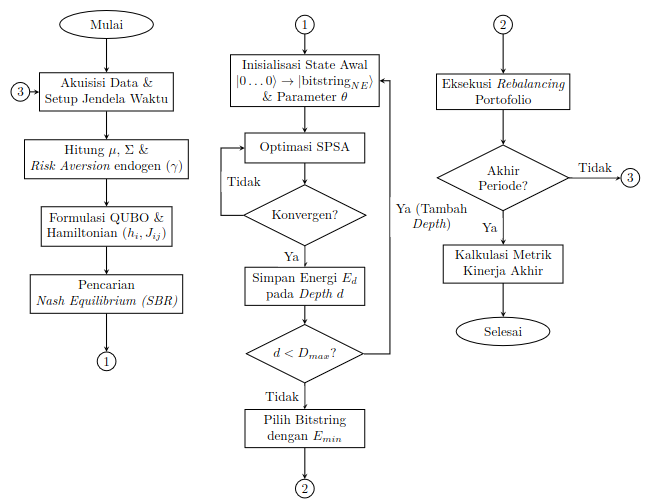
\includegraphics[width=0.6\textwidth]{Gambar/31_Dialir.png}
\end{frame}

% Slide 13: Bab 3.2 - Akuisisi dan Pra-pemrosesan Data
\begin{frame}[fragile]{Bab 3.2 - Akuisisi dan Pra-pemrosesan Data}
    \begin{algorithm}[H]
        \footnotesize
        \begin{algorithmic}[1]
            \Procedure{DataPreprocessing}{tickers, $t_{start}, t_{end}$}
                \State $\mathbf{P} \gets \text{DownloadClosingPrice}(tickers)$
                \State $r_{log} \gets \ln(\mathbf{P}_{t} / \mathbf{P}_{t-1})$ \Comment{Kalkulasi \textit{Log Return}}
                \State $\mu_{log} \gets \text{Mean}(r_{log}) - 0.5 \cdot \text{Var}(r_{log})$ \Comment{\textit{Volatility Drag}}
                \State $\Sigma \gets \text{Covariance}(r_{log})$
                \State $\gamma \gets \text{ComputeEndogenousLambda}(\mu_{log}, \Sigma)$
                \State \Return $\mu_{log}, \Sigma, \gamma$
            \EndProcedure
        \end{algorithmic}
    \end{algorithm}
\end{frame}

% Slide 14: Bab 3.3 - Pemodelan Hamiltonian Portofolio
\begin{frame}[fragile]{Bab 3.3 - Pemodelan Hamiltonian Portofolio}
    \begin{algorithm}[H]
        \footnotesize
        \begin{algorithmic}[1]
            \Procedure{BuildHamiltonian}{$\mu, \Sigma, \gamma, K, \lambda$}
                \State $Q_{ii} \gets \frac{\gamma \Sigma_{ii}}{2K^2} - \frac{\mu_i}{K} + \lambda(1 - 2K)$
                \State $Q_{ij} \gets \frac{\gamma \Sigma_{ij}}{2K^2} + \lambda$
                \State $h_i \gets -\frac{1}{2} (Q_{ii} + \sum_{j \neq i} Q_{ij}), \quad J_{ij} \gets \frac{1}{4} Q_{ij}$
                \State $H \gets \sum h_i \hat{Z}_i + \sum J_{ij} \hat{Z}_i \hat{Z}_j + C \cdot I$
                \State \Return $H$
            \EndProcedure
        \end{algorithmic}
    \end{algorithm}
\end{frame}

% Slide 15: Bab 3.4 - Algoritma Nash Sequential Best Response
\begin{frame}[fragile]{Bab 3.4 - Algoritma Nash Sequential Best Response}
    \begin{algorithm}[H]
        \scriptsize
        \begin{algorithmic}[1]
            \Procedure{NashSBR}{$\mu, \Sigma, \gamma, N, K$}
                \State $x \gets \text{InitialSelection}(K)$
                \For{$iter = 1$ to $max\_iter$}
                    \For{$i \in S_{in}$ and $j \in S_{out}$}
                        \State $x' \gets \text{Swap}(x, i, j)$
                        \If{$\Phi(x') > \Phi(x)$}
                            \State $x \gets x', \Phi \gets \Phi', improved \gets \text{True}$
                            \State \textbf{break}
                        \EndIf
                    \EndFor
                    \If{not $improved$} \textbf{break} \EndIf
                \EndFor
                \State \Return $x$ \Comment{Warm-start Bitstring}
            \EndProcedure
        \end{algorithmic}
    \end{algorithm}
\end{frame}

% Slide 16: Bab 3.5 - Optimasi Variasional HE-VQE Adaptif
\begin{frame}[fragile]{Bab 3.5 - Optimasi Variasional HE-VQE Adaptif}
    \begin{algorithm}[H]
        \scriptsize
        \begin{algorithmic}[1]
            \Procedure{AdaptiveVQE}{$H, x_{NE}, D_{max}, \lambda_{target}$}
                \State $\theta \gets \text{InitialParameters}(x_{NE})$
                \For{$d = 1$ to $D_{max}$}
                    \For{$k = 1$ to $N_{iter}$}
                        \State $\lambda_k \gets \text{PenaltyAnnealing}(k)$
                        \State $\mathcal{L}(\theta) \gets \langle \psi(\theta) | H_{obj} + \lambda_k H_{pen} | \psi(\theta) \rangle$
                        \State $\theta \gets \theta - a_k \cdot \text{SPSA\_Gradient}(\mathcal{L}, \theta)$
                    \EndFor
                    \State $\theta \gets \text{LayerExpansion}(\theta)$
                    \If{$\text{Converged}(\theta)$} \textbf{break} \EndIf
                \EndFor
                \State \Return $x^* \gets \text{Argmax}(|\langle x | \psi(\theta_{final}) \rangle|^2)$
            \EndProcedure
        \end{algorithmic}
    \end{algorithm}
\end{frame}

% Slide 17: Bab 3.6 - Simulasi Backtesting dan Metrik Evaluasi
\begin{frame}[fragile]{Bab 3.6 - Simulasi Backtesting dan Metrik Evaluasi}
    \begin{algorithm}[H]
        \scriptsize
        \begin{algorithmic}[1]
            \Procedure{BacktestLoop}{$Data, K$}
                \For{$t \in \text{Timeline}$}
                    \State $\mu, \Sigma, \gamma \gets \text{DataPreprocessing}(Data_{train})$
                    \State $H \gets \text{BuildHamiltonian}(\mu, \Sigma, \gamma, K)$
                    \State $x_{NE} \gets \text{NashSBR}(\mu, \Sigma, \gamma, K)$
                    \State $x^*_t \gets \text{AdaptiveVQE}(H, x_{NE})$
                    \State $R_t \gets \text{ExecuteRebalance}(x^*_t)$
                \EndFor
                \State \Return $\text{PerformanceMetrics}$
            \EndProcedure
        \end{algorithmic}
    \end{algorithm}
\end{frame}

% Slide 18: Bab 3.7 - Validasi Solusi Eksak Brute Force
\begin{frame}[fragile]{Bab 3.7 - Validasi Solusi Eksak Brute Force}
    \begin{algorithm}[H]
        \footnotesize
        \begin{algorithmic}[1]
            \Procedure{BruteForceValidation}{$H, N, K$}
                \State $best\_energy \gets \infty$
                \For{each $x \in \text{Combinations}(N, K)$}
                    \State $E \gets \text{CalculateIsingEnergy}(x, H)$
                    \If{$E < best\_energy$}
                        \State $best\_energy \gets E, best\_x \gets x$
                    \EndIf
                \EndFor
                \State \Return $best\_x, best\_energy$
            \EndProcedure
        \end{algorithmic}
    \end{algorithm}
\end{frame}

%%\section{Hasil dan Pembahasan}

% Slide 19: Bab 4.1.1 - Akuisisi dan Transformasi Data Numerik
\begin{frame}{Bab 4.1.1 - Akuisisi dan Transformasi Data Numerik}
    \begin{itemize}
        \item \textbf{Data Sampel (BBCA):} Kenaikan harga dari 4515,50 ke 4869,32 (Jan 2021).
        \item \textbf{Kalkulasi Imbal Hasil:}
        \begin{itemize}
            \item \textbf{Simple Return ($R$):} $\frac{4869,32 - 4515,50}{4515,50} \approx 0,0783$
            \item \textbf{Log Return ($r$):} $\ln(1 + 0,0783) \approx 0,0754$
        \end{itemize}
        \item \textbf{Justifikasi Pemilihan:}
        \begin{itemize}
            \item $R$ digunakan untuk $\mu$ guna menjaga linearitas portofolio ($r_{true} \approx \hat{r}_p + \frac{1}{2}\text{Var}(R)$).
            \item $r$ digunakan untuk $\Sigma$ guna menjamin stasioneritas runtun waktu.
        \end{itemize}
    \end{itemize}
\end{frame}

% Slide 19b: Bab 4.1.2 - Matriks Kovariansi dan Risk Aversion
\begin{frame}{Bab 4.1.2 - Matriks Kovariansi dan Risk Aversion}
    \begin{itemize}
        \item \textbf{Matriks Kovariansi ($N=2$):}
        \begin{equation*}
            \Sigma_{N2} = \begin{pmatrix} 0,0171 & 0,0022 \\ 0,0022 & 0,0225 \end{pmatrix}
        \end{equation*}
        \item \textbf{Parameter Risk Aversion Endogen ($\gamma$):}
        \begin{itemize}
            \item Rasio Sharpe Agregat ($Z$): $\bar{\mu}_l / \bar{\sigma}_l = 0,1330 / 0,2221 \approx 0,5988$.
            \item Fungsi Sigmoid: $\gamma = 1 / (1 + e^Z) \approx \mathbf{0,3547}$.
        \end{itemize}
        \item \textbf{Interpretasi:} Nilai $\gamma$ rendah mencerminkan optimisme pasar pada jendela awal, memicu alokasi kapital yang lebih berani.
    \end{itemize}
\end{frame}

% Slide 20: Bab 4.2 - Formulasi EPG dan Hasil Nash
\begin{frame}{Bab 4.2 - Formulasi EPG dan Hasil Nash}
    \begin{itemize}
        \item \textbf{Insentif Marginal ($\Delta \Phi$):}
        \begin{equation*}
            \Delta \Phi(\vec{x}) = \frac{\mu_i}{k} - \frac{\gamma \sigma_i^2}{2k^2} - \gamma \sum_{j < i} \sigma_{ij} \frac{x_j}{k^2}
        \end{equation*}
        \item \textbf{Hasil Pencarian Nash Equilibrium ($N=2$):}
    \end{itemize}
    \begin{table}
        \footnotesize
        \centering
        \begin{tabular}{cc|c|c|}
        \cline{3-4}
        & & \multicolumn{2}{c|}{Aset TLKM ($x_2$)} \\ \cline{3-4}
        & & Status 0 & Status 1 \\ \hline
        \multicolumn{1}{|c|}{\multirow{2}{*}{Aset BBCA ($x_1$)}} & Status 0 & (0, 0) & (0, 0,1183) \\ \cline{2-4} 
        \multicolumn{1}{|c|}{} & Status 1 & \textbf{(0,1909, 0)} & (0,1901, 0,1175) \\ \hline
        \end{tabular}
        \caption{Nash Equilibrium tercapai pada $|10\rangle$ (Hanya BBCA terpilih).}
    \end{table}
\end{frame}

% Slide 21: Bab 4.3 - Derivasi EPG ke Hamiltonian Ising
\begin{frame}{Bab 4.3 - Derivasi EPG ke Hamiltonian Ising}
    \begin{itemize}
        \item \textbf{Langkah Transformasi:}
        \begin{enumerate}
            \item Definisikan fungsi energi: $E(\vec{x}) = -\Phi(\vec{x})$.
            \item Substitusi variabel biner ke spin: $x_i = (1 - s_i)/2$.
            \item Ekstraksi koefisien Pauli-Z ($\hat{Z}$).
        \end{enumerate}
        \item \textbf{Hasil Hamiltonian Numerik (Jan 2021):}
        \begin{equation*}
            \hat{\mathcal{H}}_{N2} \approx 0,0915 \hat{Z}_1 + 0,0533 \hat{Z}_2 + 0,5022 \hat{Z}_1 \hat{Z}_2 - 0,1470
        \end{equation*}
        \item \textbf{Analisis:} Koefisien interaksi didominasi oleh pinalti anggaran $A \approx 0,5$, menjamin validitas solusi kardinalitas.
    \end{itemize}
\end{frame}

% Slide 22: Bab 4.4 - Sirkuit Kuantum dan Gradien Energi
\begin{frame}{Bab 4.4 - Sirkuit Kuantum dan Gradien Energi}
    \begin{columns}
        \begin{column}{0.55\textwidth}
            \begin{itemize}
                \item \textbf{Konstruksi State:} $\ket{\psi(\boldsymbol{\theta})} = \hat{U}_{ent} \hat{U}_{rot}(\boldsymbol{\theta}) \ket{0\dots0}$.
                \item \textbf{Gradien Energi:} Dicari untuk meminimalkan $\langle \hat{\mathcal{H}} \rangle$:
                \begin{equation*}
                    \nabla_{\theta} E = \frac{\partial}{\partial \theta} \langle \psi(\theta) | \hat{H} | \psi(\theta) \rangle
                \end{equation*}
                \item \textbf{Sinergi:} Kombinasi gerbang rotasi $R_y, R_z$ dan keterbelitan CNOT membentuk lanskap energi yang dapat dilatih.
            \end{itemize}
        \end{column}
        \begin{column}{0.45\textwidth}
            \begin{figure}
                \centering
                
\includegraphics[width=\textwidth]{Hasil_N2_GT/Analisis_Window_N2/2021-05-05_circuit.png}
                \caption{Arsitektur HEA sistem N=2.}
            \end{figure}
        \end{column}
    \end{columns}
\end{frame}

% Slide 23: Bab 4.5 - Penurunan Parameter Shift Rule (PSR)
\begin{frame}{Bab 4.5 - Penurunan Parameter Shift Rule (PSR)}
    \begin{itemize}
        \item \textbf{Aksioma:} Generator gerbang kuantum seringkali memiliki dua nilai eigen unik ($\pm r$).
        \item \textbf{Derivasi:} Ekspansi uniter gerbang rotasi $U(\theta) = e^{-i\theta G}$.
    \end{itemize}
    \begin{equation*}
        \frac{\partial E}{\partial \theta} = \frac{1}{2} \left[ E\left(\theta + \frac{\pi}{2}\right) - E\left(\theta - \frac{\pi}{2}\right) \right]
    \end{equation*}
    \begin{itemize}
        \item \textbf{Signifikansi:} Memberikan nilai gradien yang identik dengan turunan analitik tanpa limit $\epsilon \to 0$.
    \end{itemize}
\end{frame}

% Slide 24: Bab 4.6 - Derivasi dan Iterasi Numerik SPSA
\begin{frame}{Bab 4.6 - Derivasi dan Iterasi Numerik SPSA}
    \begin{itemize}
        \item \textbf{Ekspansi Taylor Orde-2:} SPSA membatalkan suku orde genap melalui selisih evaluasi maju-mundur ($E_+ - E_-$).
        \item \textbf{Estimator Gradien:} $\hat{g}_i = (E_+ - E_-) / (2 c_k \Delta_i)$.
        \item \textbf{Contoh Satu Langkah Iterasi:}
        \begin{itemize}
            \item \textbf{Input:} $\theta^{(0)} = [\pi/2, \pi/2]$, $\Delta_k = [1, -1]$.
            \item \textbf{Output:} $\Delta E = -0,0076 \rightarrow \hat{g} = [-0,038, 0,038]^T$.
            \item \textbf{Update:} $\theta^{(1)} = \theta^{(0)} - 0,1\hat{g} = [1,5746, 1,5670]^T$.
        \end{itemize}
    \end{itemize}
\end{frame}

% Slide 25: Bab 4.7 - Evolusi Entropi: Shannon ke Von Neumann
\begin{frame}{Bab 4.7 - Evolusi Entropi: Shannon ke Von Neumann}
    \begin{itemize}
        \item \textbf{Shannon ($H$):} Ketidakpastian informasi klasik $-\sum p_i \log_2 p_i$.
        \item \textbf{Von Neumann ($S$):} Perluasan ke operator densitas kuantum $\rho$:
    \end{itemize}
    \begin{equation*}
        S(\rho) = -\text{Tr}(\rho \log \rho) = -\sum_i \lambda_i \log \lambda_i
    \end{equation*}
    \begin{itemize}
        \item \textbf{Studi Kasus Jendela 1:}
        \begin{itemize}
            \item \textbf{N=2:} Probabilitas status optimal 0,98 $\rightarrow S = 0,1414$ bit.
            \item \textbf{N=4:} Probabilitas status optimal 0,94 $\rightarrow S = 0,3274$ bit.
        \end{itemize}
    \end{itemize}
\end{frame}

% Slide 26: Bab 4.8 - Analisis Barren Plateau dan Warm-Start
\begin{frame}{Bab 4.8 - Analisis Barren Plateau dan Warm-Start}
    \begin{itemize}
        \item \textbf{Jebakan Gradien:} Variansi gradien menyusut drastis pada sistem $N=4$ saat kedalaman $L > 5$.
        \item \textbf{Expressibility vs Trainability:} Peningkatan kapasitas sirkuit seringkali mengorbankan kemudahan optimasi.
    \end{itemize}
    \begin{center}
        
\includegraphics[width=0.7\textwidth]{Hasil_N4_GT/grafik_depth_per_window_N4.png} \\
        \footnotesize \textit{Visualisasi pemilihan depth optimal menggunakan inisialisasi Nash.}
    \end{center}
    \begin{itemize}
        \item \textbf{Observasi:} Inisialisasi EPG memandu sirkuit ke sub-ruang Hilbert yang bermakna, menjaga gradien tetap terdeteksi.
    \end{itemize}
\end{frame}

% Slide 27: Bab 4.9 - Validasi Brute Force dan Benchmark SLSQP
\begin{frame}{Bab 4.9 - Validasi Brute Force dan Benchmark SLSQP}
    \begin{itemize}
        \item \textbf{Brute Force (N=2):}
        \begin{itemize}
            \item $E(|10\rangle) = -0,1909$ (Global Minimum).
            \item $E(|00\rangle) = 4,1972$ (Forbidden State).
        \end{itemize}
        \item \textbf{SLSQP:} Algoritma optimasi kontinu dengan diskritisasi \textit{Top-K}.
    \end{itemize}
    \begin{exampleblock}{Fair Comparison}
        Kedua metode diuji pada parameter batasan yang identik guna membandingkan efisiensi alokasi modal hibrida secara objektif.
    \end{exampleblock}
\end{frame}

% Slide 28: Bab 4.10 - Analisis Performa Portofolio (Hasil Utama)
\begin{frame}{Bab 4.10 - Analisis Performa Portofolio (Hasil Utama)}
    \begin{table}
        \scriptsize
        \centering
        \begin{tabular}{|l|c|c|c|c|c|c|}
        \hline
        \multirow{2}{*}{\textbf{Strategi}} & \multicolumn{3}{c|}{\textbf{Sistem N=2}} & \multicolumn{3}{c|}{\textbf{Sistem N=4}} \\ \cline{2-7} 
         & \textbf{Return} & \textbf{Sharpe} & \textbf{MDD} & \textbf{Return} & \textbf{Sharpe} & \textbf{MDD} \\ \hline
        \textbf{GT-VQE (Hibrida)} & \textbf{51,34\%} & \textbf{0,7357} & 15,91\% & \textbf{73,15\%} & \textbf{1,0107} & \textbf{16,68\%} \\ \hline
        VQE (Tanpa GT) & 43,21\% & 0,6471 & 15,91\% & 16,89\% & 0,3592 & 20,89\% \\ \hline
        SLSQP (Klasik) & 51,34\% & 0,6736 & 15,91\% & 12,91\% & 0,2810 & 21,12\% \\ \hline
        Equal Weight & 37,29\% & 0,6848 & 14,62\% & 35,57\% & 0,6790 & 18,42\% \\ \hline
        \end{tabular}
        \caption{GT-VQE mendominasi seluruh metrik pada dimensi sistem yang lebih besar (N=4).}
    \end{table}
\end{frame}

% Slide 30: Bab 4.11 - Dinamika Rebalancing Jendela Ekstrem
\begin{frame}{Bab 4.11 - Dinamika Rebalancing Jendela Ekstrem}
    \begin{itemize}
        \item \textbf{Agilitas Portofolio:} Transisi status $|10\rangle \to |01\rangle$ secara instan merespons lonjakan risiko BBCA (Feb-Mar 2021).
    \end{itemize}
    \begin{figure}
        \centering
        \begin{subfigure}[b]{0.45\textwidth}
            \centering
            
\includegraphics[width=\textwidth]{Hasil_N2_GT/Analisis_Window_N2/2021-02-02_window.png}
            \caption{Jan-Feb 2021 (Aset BBCA)}
        \end{subfigure}
        \hfill
        \begin{subfigure}[b]{0.45\textwidth}
            \centering
            
\includegraphics[width=\textwidth]{Hasil_N2_GT/Analisis_Window_N2/2021-03-04_window.png}
            \caption{Mar-Apr 2021 (Aset TLKM)}
        \end{subfigure}
        \caption{Quantum rebalancing mendeteksi pergeseran energi Hamiltonian pasar.}
    \end{figure}
\end{frame}

%%\section{Penutup}

% Slide 31: Bab 5.1 - Kesimpulan (1)
\begin{frame}{Bab 5.1 - Kesimpulan: Formulasi EPG-Hamiltonian}
    \begin{itemize}
        \item \textbf{Integrasi Teori-Fisis:} Formulasi Markowitz ke dalam kerangka \textit{Exact Potential Game} (EPG) berhasil memetakan utilitas ekonomi menjadi sistem Hamiltonian fisis secara konsisten.
        \item \textbf{Presisi Parameter:}
        \begin{itemize}
            \item \textbf{Log Return:} Menjaga simetri interaksi risiko ($J_{ij}$) tanpa distorsi matematis.
            \item \textbf{Simple Return:} Mempertahankan linearitas bias ekspektasi imbal hasil ($h_i$).
        \end{itemize}
        \item \textbf{Integritas Solusi:} Implementasi suku penalti anggaran ($A$) efektif mencegah sirkuit kuantum terjebak pada status yang melanggar batasan investasi.
    \end{itemize}
\end{frame}

% Slide 32: Bab 5.1 - Kesimpulan (2)
\begin{frame}{Bab 5.1 - Kesimpulan: Efektivitas Warm-Start Nash}
    \begin{itemize}
        \item \textbf{Akselerasi Konvergensi:} Penerapan ekuilibrium nash sebagai inisialisasi \textit{warm-start} meningkatkan stabilitas konvergensi algoritma VQE secara signifikan.
        \item \textbf{Mitigasi Barren Plateaus:} Injeksi solusi strategis memandu sirkuit melewati area kelenyapan varians gradien.
        \item \textbf{Efisiensi Sumber Daya:} Algoritma mampu mencapai \textit{ground state} pada kedalaman sirkuit dangkal ($L=2$ hingga $L=3$), mereduksi beban komputasi sirkuit kuantum.
    \end{itemize}
\end{frame}

% Slide 33: Bab 5.1 - Kesimpulan (3)
\begin{frame}{Bab 5.1 - Kesimpulan: Kapabilitas dan Performa}
    \begin{itemize}
        \item \textbf{Ketangguhan Stokastik:} Sinergi arsitektur HEA dan optimizer SPSA menunjukkan kapabilitas tinggi dalam menangani volatilitas pasar modal.
        \item \textbf{Agilitas Rebalancing:} Estimasi gradien simultan memungkinkan respons cepat terhadap pergeseran ekuilibrium pasar.
        \item \textbf{Superioritas Empiris:} Strategi GT-VQE menghasilkan pertumbuhan modal paling unggul dengan \textbf{Sharpe Ratio 1,0107} (N=4), melampaui performa algoritma klasik SLSQP.
    \end{itemize}
\end{frame}

% Slide 34: Bab 5.2 - Saran Pengembangan
\begin{frame}{Bab 5.2 - Saran Pengembangan}
    \begin{enumerate}
        \item \textbf{Parameter Noise:} Integrasi model dekoherensi qubit dan \textit{gate fidelity} untuk implementasi pada perangkat keras kuantum riil.
        \item \textbf{Eksplorasi Arsitektur:} Pengujian variasi sirkuit \textit{ansatz} lain dan algoritma optimasi hibrida untuk meningkatkan laju konvergensi.
        \item \textbf{Analisis Krisis:} Perluasan data pada periode fenomena \textit{Black Swan} guna menguji reliabilitas algoritma dalam mempertahankan stabilitas ekuilibrium di tengah guncangan ekstrem.
    \end{enumerate}
    \vspace{0.8cm}
    \begin{center}
        \huge \textbf{Terima Kasih} \\
        \medskip
        \large Ada Pertanyaan?
    \end{center}
\end{frame}


\end{document}
